% Asset ID: A21IntegrationTikZ-003
\documentclass[tikz,border=8pt]{standalone}
\usepackage{amsmath}
\usepackage{tikz}
\begin{document}
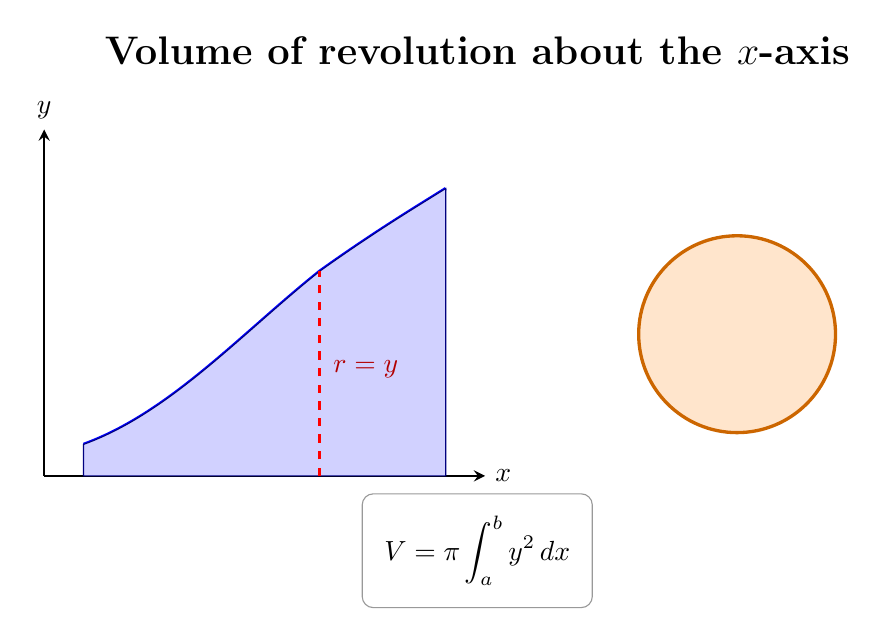
\begin{tikzpicture}[x=1cm,y=1cm,>=stealth]
\node[font=\Large\bfseries] at (6,6.4) {Volume of revolution about the $x$-axis};
\draw[->, thick] (0.5,1) -- (6.1,1) node[right] {$x$};
\draw[->, thick] (0.5,1) -- (0.5,5.4) node[above] {$y$};
\draw[blue, very thick] (1,1.4) .. controls (2.1,1.8) and (3.0,2.8) .. (4.0,3.6) .. controls (4.7,4.1) and (5.2,4.4) .. (5.6,4.65);
\path[fill=blue!18, draw=blue!50!black] (1,1) -- (1,1.4) .. controls (2.1,1.8) and (3.0,2.8) .. (4.0,3.6) .. controls (4.7,4.1) and (5.2,4.4) .. (5.6,4.65) -- (5.6,1) -- cycle;
\draw[red, very thick, dashed] (4,1) -- (4,3.6);
\node[right, red!70!black] at (4.05,2.35) {$r=y$};
\draw[orange!80!black, very thick, fill=orange!20] (9.3,2.8) circle (1.25);
\node[draw=black!40, fill=white, rounded corners, inner sep=8pt] at (6,0.05)
{$\displaystyle V=\pi\int_a^b y^2\,dx$};
\end{tikzpicture}
\end{document}